\subsection{Разработка архитектуры программного средства}
\label{sec:design:architecture}

Как было указано в пункте \ref{sec:analysis:requirements:language}, на основании анализа вариантов проектирования приложения для различных платформ, 
было принято решение выбрать основной для разработки настольное приложение с небольшим веб-сервисом координатором.

Одним из вариантов архитектуры для приложений данного типа является двухзвенная клиент-серверная архитектура представленная на рисунке \ref{sec:design:architecture:client_server}. 
В проектируемом приложении задачами сервера будет являтся координация клиентов и помощь в установке интернет соединения на основе протокола TCP, что позволит достичь максимально
возможного уровня надежности данных, хоть и с недостатками в виде сниженной скорости передачи данных. Задачей сервера будет возврат запрашиваемых данных по запросу клиентов, отправка команд игрокам, а также хранение небольшой локальной таблицы со списком игровых лобби.
По этой причине необходимость в базе данных отпадает -- так как большого объема данных не будет и ценность хранимых данных невысока. В дополнение стоит сказать, что доступ к локальному хранилищу быстрее, чем к бд.
Выбранная в пункте \ref{sec:analysis:requirements:language} программная платформа позволяет нам это реализовать.

\begin{figure}[ht]
\centering
	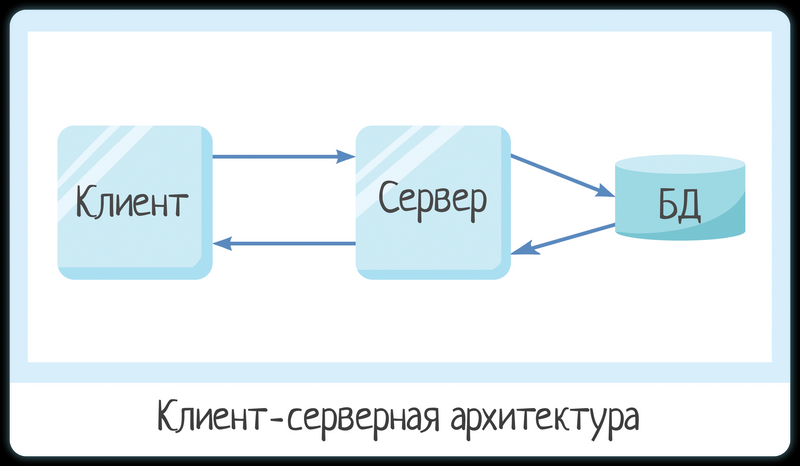
\includegraphics[scale=0.7]{attachments/client_server.png}
	\caption{Типичная двухзвенная архитектура}
	\label{sec:design:architecture:client_server}
\end{figure}

В свою очередь задача клиентской части при взаимодействии с сервером состоит в том, чтобы при создании игрового лобби передать на сервер информацию о лобби, 
а также о сети, в которой находится машина-хост. Это нужно для того, чтобы другой клиент, который хочет подключится к игре мог воспользоваться координатором и принимать участие в игровом процессе.
В данном случае сервер является своеобразным валидатором игровых действий и хранит всегда валидные состояния, что повышает надежность разрабатываемого программного обеспечения, 
а также позволяет без лишних усилий реализовать некоторый функционал, например, подключение посреди игры. Общение между клиентами будет проходить посредством комманд, которые будут
выполяться на сервере и рассылатся клиентам для локального выполнения.

В итоге архитектура, по которой будут работать клиенты и сервер-координатор выглядит следущим образом (рис. \ref{sec:design:architecture:p2p}). В центре находится сервер-координатор, 
все остальные компьютеры -- клиенты.

\begin{figure}[ht]
\centering
    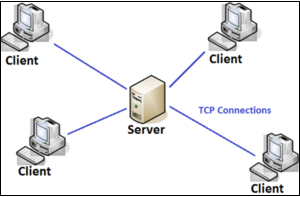
\includegraphics[scale=2]{attachments/p2p.png}
    \caption{Архитектура клиент-сервер}
    \label{sec:design:architecture:p2p}
\end{figure}